%!TEX root = ../thesis.tex
\section{Hardware}
\label{sec:pastwork:hardware}

% ~\cite{Li:2011ur,Li:2010en,Zhang:2009dp}

Different approaches are available for 3D imaging including laser scanning~\cite{Blais:1988te}, viewpoint reconstruction~\cite{Hartley:2000un} and structured light scanning~\cite{Halioua:1984ue}. Structured light scanning, compared to other approaches, is fast and accurate. For palmprint recognition, speed is an important factor. The verification or identification result must be given in a short time. Otherwise the system is barely suitable for real-world applications.

% http://en.wikipedia.org/wiki/Structured-light_3D_scanner

If a surface is not flat, a narrow band of light would appear distorted when projected onto the shaped surface when viewing from any perspective other than that of the projector. And the geometry of part the 3D surface lit by the projected strip can be reconstructed by using the measured distortion.

The bands of light can be projected one after another. Or, to be faster and more efficient, patterns of a group of strips can be projected all at once so that a multitude of samples can be simultaneously acquired. The distortion of the pattern, when seen from a different viewpoint other than that of the projector, can be used to reconstruct the entire geometry of the 3D surface.

\begin{figure}[htb]
\begin{center}
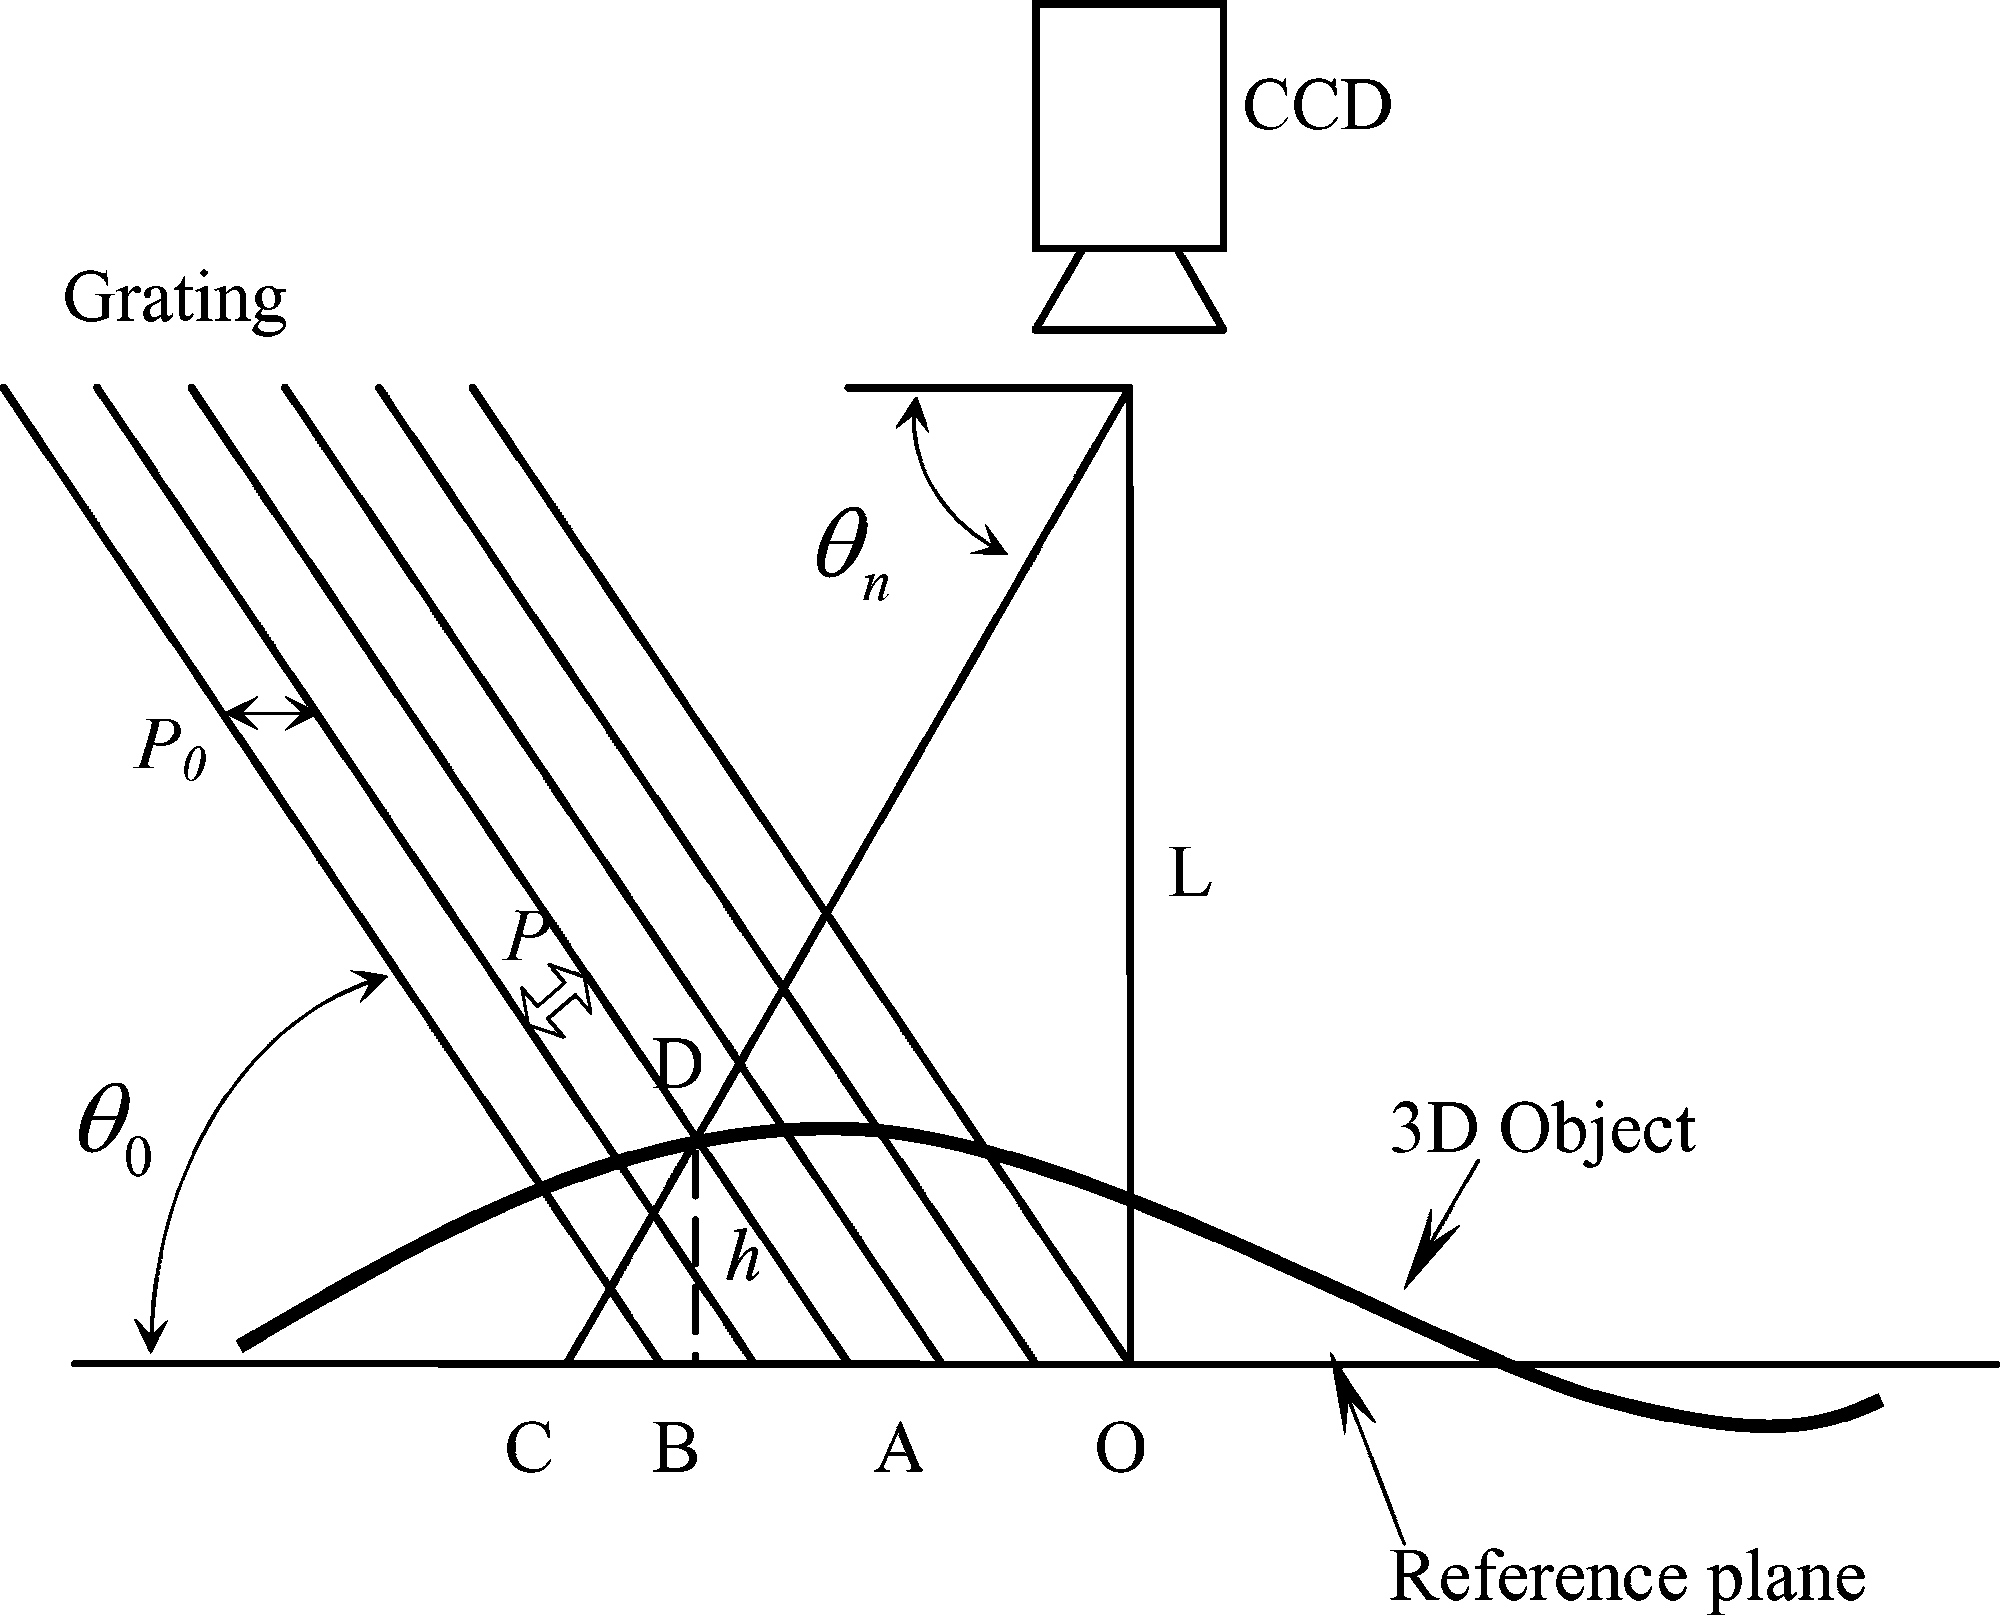
\includegraphics[width=0.9\linewidth]{ch-pastwork/figures/sli}
\caption[The principle of structured-light imaging]{The principle of structured-light imaging\cite{Li:2009eq}}
\label{fig:pastwork:sli}
\end{center}
\end{figure}

Various patterns of strips are possible, among which patterns of parallel structured light stripes projection are widely used. Figure~\ref{fig:pastwork:strippattern} shows the geometrical deformation of a strip pattern projected onto a palm. An exact recovery of 3D coordinates can be retrieved by applying calculations on the displacement of the stripes. Precision of this approach has been proved to be the best available.

\begin{figure}[htb]
\begin{center}
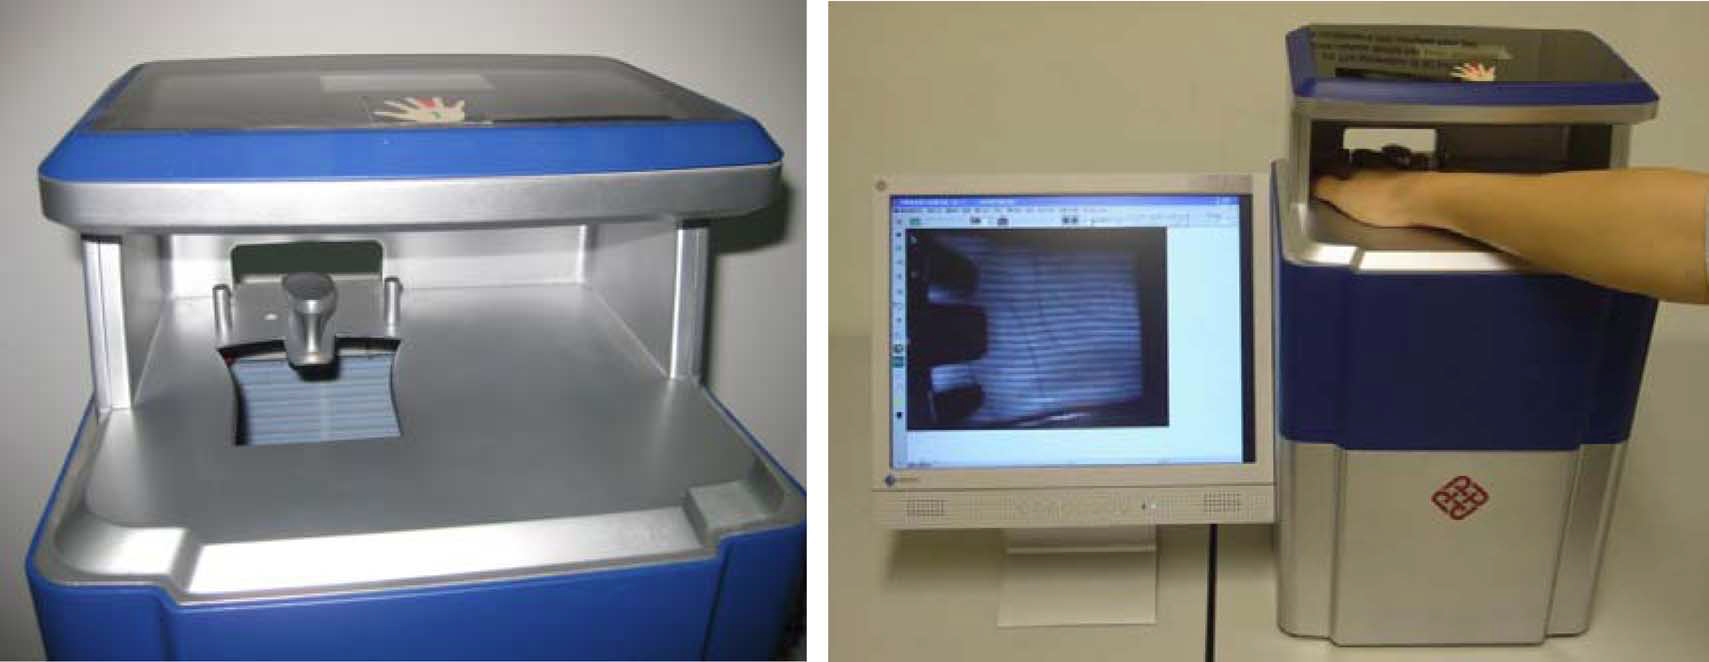
\includegraphics[width=0.9\linewidth]{ch-pastwork/figures/device}
\caption{3D palmprint capturing device}
\label{fig:pastwork:device}
\end{center}
\end{figure}

Figure ~\ref{fig:pastwork:device} shows the 3D palmprint capturing device designed by David et al. ~\cite{Zhang:2008kc}. The system proposed has a resolution of 768x576.

\begin{figure}[htb]
\begin{center}
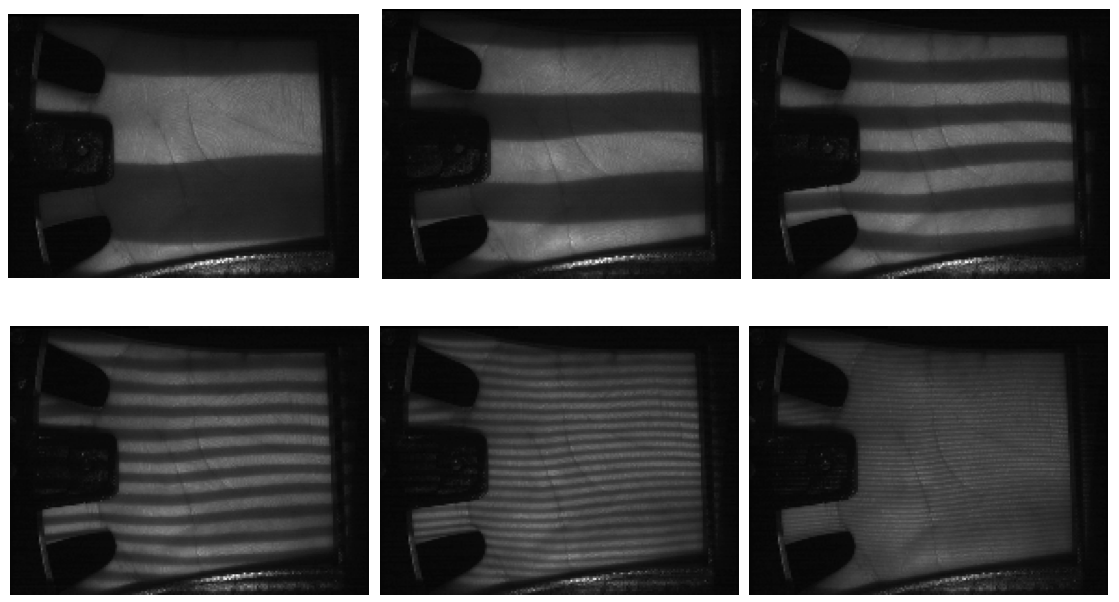
\includegraphics[width=0.9\linewidth]{ch-pastwork/figures/strippattern}
\caption[Parallel pattern of the stripes projected on a palm sample]{Parallel pattern of the stripes projected on a palm sample~\cite{Li:2009eq}}
\label{fig:pastwork:strippattern}
\end{center}
\end{figure}

